\documentclass[11pt,compress,t,notes=noshow, xcolor=table]{beamer}
\usepackage[]{graphicx}\usepackage[]{color}
% maxwidth is the original width if it is less than linewidth
% otherwise use linewidth (to make sure the graphics do not exceed the margin)
\makeatletter
\def\maxwidth{ %
  \ifdim\Gin@nat@width>\linewidth
    \linewidth
  \else
    \Gin@nat@width
  \fi
}
\makeatother

\newcommand{\citebutton}[2]{%
\beamergotobutton{\href{#2}{#1}}%
}

\newcommand{\blu}[1]{\textcolor{blue}{#1}}
\newcommand{\org}[1]{\textcolor{orange}{#1}}
\newcommand{\ques}{\textbf{\textcolor{red}{Question:  }}}
\newcommand{\questionssofar}{\begin{frame}\frametitle{Any questions?}\end{frame}}

\newcommand\warning{%
 \makebox[1.4em][c]{%
 \makebox[0pt][c]{\raisebox{.1em}{\scriptsize!}}%
 \makebox[0pt][c]{\color{red}\normalsize$\bigtriangleup$}}}%

\definecolor{fgcolor}{rgb}{0.345, 0.345, 0.345}
\newcommand{\hlnum}[1]{\textcolor[rgb]{0.686,0.059,0.569}{#1}}%
\newcommand{\hlstr}[1]{\textcolor[rgb]{0.192,0.494,0.8}{#1}}%
\newcommand{\hlcom}[1]{\textcolor[rgb]{0.678,0.584,0.686}{\textit{#1}}}%
\newcommand{\hlopt}[1]{\textcolor[rgb]{0,0,0}{#1}}%
\newcommand{\hlstd}[1]{\textcolor[rgb]{0.345,0.345,0.345}{#1}}%
\newcommand{\hlkwa}[1]{\textcolor[rgb]{0.161,0.373,0.58}{\textbf{#1}}}%
\newcommand{\hlkwb}[1]{\textcolor[rgb]{0.69,0.353,0.396}{#1}}%
\newcommand{\hlkwc}[1]{\textcolor[rgb]{0.333,0.667,0.333}{#1}}%
\newcommand{\hlkwd}[1]{\textcolor[rgb]{0.737,0.353,0.396}{\textbf{#1}}}%
\let\hlipl\hlkwb

\usepackage{framed}
\makeatletter
\newenvironment{kframe}{%
 \def\at@end@of@kframe{}%
 \ifinner\ifhmode%
  \def\at@end@of@kframe{\end{minipage}}%
  \begin{minipage}{\columnwidth}%
 \fi\fi%
 \def\FrameCommand##1{\hskip\@totalleftmargin \hskip-\fboxsep
 \colorbox{shadecolor}{##1}\hskip-\fboxsep
     % There is no \\@totalrightmargin, so:
     \hskip-\linewidth \hskip-\@totalleftmargin \hskip\columnwidth}%
 \MakeFramed {\advance\hsize-\width
   \@totalleftmargin\z@ \linewidth\hsize
   \@setminipage}}%
 {\par\unskip\endMakeFramed%
 \at@end@of@kframe}
\makeatother

\definecolor{shadecolor}{rgb}{.97, .97, .97}
\definecolor{messagecolor}{rgb}{0, 0, 0}
\definecolor{warningcolor}{rgb}{1, 0, 1}
\definecolor{errorcolor}{rgb}{1, 0, 0}
\newenvironment{knitrout}{}{} % an empty environment to be redefined in TeX

\usepackage{alltt}
\newcommand{\SweaveOpts}[1]{}  % do not interfere with LaTeX
\newcommand{\SweaveInput}[1]{} % because they are not real TeX commands
\newcommand{\Sexpr}[1]{}       % will only be parsed by R
\newcommand{\xmark}{\ding{55}}%


\usepackage[english]{babel}
\usepackage[utf8]{inputenc}

\usepackage{dsfont}
\usepackage{verbatim}
\usepackage{amsmath}
\usepackage{amsfonts}
\usepackage{amssymb}
\usepackage{bm}
\usepackage{csquotes}
\usepackage{multirow}
\usepackage{longtable}
\usepackage{booktabs}
\usepackage{enumerate}
\usepackage[absolute,overlay]{textpos}
\usepackage{psfrag}
\usepackage{algorithm}
\usepackage{algpseudocode}
\usepackage{eqnarray}
\usepackage{arydshln}
\usepackage{tabularx}
\usepackage{placeins}
\usepackage{tikz}
\usepackage{setspace}
\usepackage{colortbl}
\usepackage{mathtools}
\usepackage{wrapfig}
\usepackage{bm}
\usepackage{amsmath}
\usepackage{pifont}

\usetikzlibrary{shapes.multipart,shapes,arrows,automata,positioning,calc,chains,trees, shadows}
\tikzset{
  %Define standard arrow tip
  >=stealth',
  %Define style for boxes
  punkt/.style={
    rectangle,
    rounded corners,
    draw=black, very thick,
    text width=6.5em,
    minimum height=2em,
    text centered},
  % Define arrow style
  pil/.style={
    ->,
    thick,
    shorten <=2pt,
    shorten >=2pt,}
}

\tikzstyle{vec}=[draw, rectangle, fill = white, minimum width=5mm, minimum height=1cm, inner sep = 2pt]

\usepackage{subfig}

% Defines macros and environments
\usepackage{../../style/lmu-lecture}


\let\code=\texttt
\let\proglang=\textsf

\setkeys{Gin}{width=0.9\textwidth}

\setbeamertemplate{frametitle}{\expandafter\uppercase\expandafter\insertframetitle}

\usepackage{bbm}
% basic latex stuff
\newcommand{\pkg}[1]{{\fontseries{b}\selectfont #1}} %fontstyle for R packages
\newcommand{\lz}{\vspace{0.5cm}} %vertical space
\newcommand{\dlz}{\vspace{1cm}} %double vertical space
\newcommand{\oneliner}[1] % Oneliner for important statements
{\begin{block}{}\begin{center}\begin{Large}#1\end{Large}\end{center}\end{block}}


%new environments
\newenvironment{vbframe}  %frame with breaks and verbatim
{
 \begin{frame}[containsverbatim,allowframebreaks]
}
{
\end{frame}
}

\newenvironment{vframe}  %frame with verbatim without breaks (to avoid numbering one slided frames)
{
 \begin{frame}[containsverbatim]
}
{
\end{frame}
}

\newenvironment{blocki}[1]   % itemize block
{
 \begin{block}{#1}\begin{itemize}
}
{
\end{itemize}\end{block}
}

\newenvironment{fragileframe}[2]{  %fragile frame with framebreaks
\begin{frame}[allowframebreaks, fragile, environment = fragileframe]
\frametitle{#1}
#2}
{\end{frame}}


\newcommand{\myframe}[2]{  %short for frame with framebreaks
\begin{frame}[allowframebreaks]
\frametitle{#1}
#2
\end{frame}}

\newcommand{\remark}[1]{
  \textbf{Remark:} #1
}


\newenvironment{deleteframe}
{
\begingroup
\usebackgroundtemplate{
\includegraphics[width=\paperwidth,height=\paperheight]{../style/color/red.png}}
 \begin{frame}
}
{
\end{frame}
\endgroup
}
\newenvironment{simplifyframe}
{
\begingroup
\usebackgroundtemplate{
\includegraphics[width=\paperwidth,height=\paperheight]{../style/color/yellow.png}}
 \begin{frame}
}
{
\end{frame}
\endgroup
}\newenvironment{draftframe}
{
\begingroup
\usebackgroundtemplate{
\includegraphics[width=\paperwidth,height=\paperheight]{../style/color/green.jpg}}
 \begin{frame}
}
{
\end{frame}
\endgroup
}
% https://tex.stackexchange.com/a/261480: textcolor that works in mathmode
\makeatletter
\renewcommand*{\@textcolor}[3]{%
  \protect\leavevmode
  \begingroup
    \color#1{#2}#3%
  \endgroup
}
\makeatother





\input{../../latex-math/basic-math.tex}
\input{../../latex-math/basic-ml.tex}

\newcommand{\titlefigure}{figure/bert.jpeg}
\newcommand{\learninggoals}{
\item Know the pre-training tasks
\item How to construct samples
\item Understand the pre-training
\item Gain understanding of the fine-tuning procedure
\item Differences between token- and sequence classification}

\title{BERT}
% \author{}
\institute{\href{https://slds-lmu.github.io/lecture_dl4nlp/}{slds-lmu.github.io/lecture\_dl4nlp}}
\date{}

\begin{document}
\lecturechapter{Pre-training \& Fine-Tuning}
\lecture{Deep Learning for NLP}

% ------------------------------------------------------------------------------

\begin{frame}{Masked Language Modeling (MLM)}

\vfill

\textbf{First remark:}

\begin{itemize}
	\item Distinguish from \textit{Masked Self-Attenion}\\ 
				$\to$ Masked Self-Attention is an architectural detail in the decoder of the Transformer, i.e. used by e.g. GPT
	\item Masked Self-Attention as a way to prevent causality issues in a Transformer decoder 
	\item MLM is a self-supervised \textit{modeling objective} introduced to couple Self-Attention and (deep) bidirectionality without violating causality
\end{itemize}

\vfill

\end{frame}

% ------------------------------------------------------------------------------

\begin{frame}{MLM (2)}

\begin{itemize}
\item \textbf{Training objective:} $$\text{Given a sentence, predict \texttt{[MASK]}ed tokens}$$
\item \textbf{Generation of samples:} $$\text{Randomly replace* a fraction of the words by \texttt{[MASK]}}$$
  \scriptsize *Sample 15\% of the tokens; replace 80\% of them by \texttt{[MASK]}, 10\% by a random token \& leave 10\% unchanged
\item \normalsize \textbf{Input:}\\\mbox{}\\
			\footnotesize
\begin{tabular}{|cccccccccc|}
\hline
The & quick & brown & \cellcolor{blue!65}\texttt{[MASK]} & jumps & over & the & \cellcolor{blue!65}\texttt{[MASK]} & dog & . \\
\hline
\end{tabular}\\\mbox{}
\item \normalsize \textbf{Targets:} $$(fox,\; lazy)$$
\end{itemize}

\end{frame}

% ------------------------------------------------------------------------------

\begin{frame}{MLM (3)}

\begin{itemize}
\item \warning But 20\% of the samples will look different!\\
			$\to$ 10\% replaced by a random token; 10\% left unchanged
\item \normalsize \textbf{Input (first case):}\\\mbox{}\\
			\footnotesize
\begin{tabular}{|cccccccccc|}
\hline
The & quick & brown & \cellcolor{blue!65}\texttt{orange} & jumps & over & the & \cellcolor{blue!65}\texttt{is} & dog & . \\
\hline
\end{tabular}\\\mbox{}
\item \normalsize \textbf{Targets (first case):} $$(fox,\; lazy)$$
\item \normalsize \textbf{Input (second case):}\\\mbox{}\\
			\footnotesize
\begin{tabular}{|cccccccccc|}
\hline
The & quick & brown & \cellcolor{blue!65}\texttt{fox} & jumps & over & the & \cellcolor{blue!65}\texttt{lazy} & dog & . \\
\hline
\end{tabular}\\\mbox{}
\item \normalsize \textbf{Targets (second case):} $$(fox,\; lazy)$$
\end{itemize}

\end{frame}
% ------------------------------------------------------------------------------

\begin{frame}{MLM (4)}

\vfill

\textbf{Discrepancy between pre-training \& fine-tuning:}

\begin{itemize}
	\item \texttt{[MASK]}-token as central part of pre-training procedure
	\item \texttt{[MASK]}-token does not occur during fine-tuning
	\item \textbf{Modified pre-training task:}\\
				Predict 15\% of the tokens of which only 80\% have been replaced by \texttt{[MASK]}
				\begin{itemize}
					\item 80\% of the selected tokens are actually \texttt{[MASK]}ed
					\item 10\% of the selected tokens: The model has to ``understand`` that the word needs to be \textit{replaced}
					\item 10\% of the selected tokens: The model has to ``understand`` that the word needs to be \textit{kept}
			\end{itemize}
	\item This ensures overlap between the kind data seen during pre-training and during fine-tuning
\end{itemize}
	
\vfill

\end{frame}

% ------------------------------------------------------------------------------

\begin{frame}{MLM (5)}

\vfill

	\begin{figure}
		\centering
		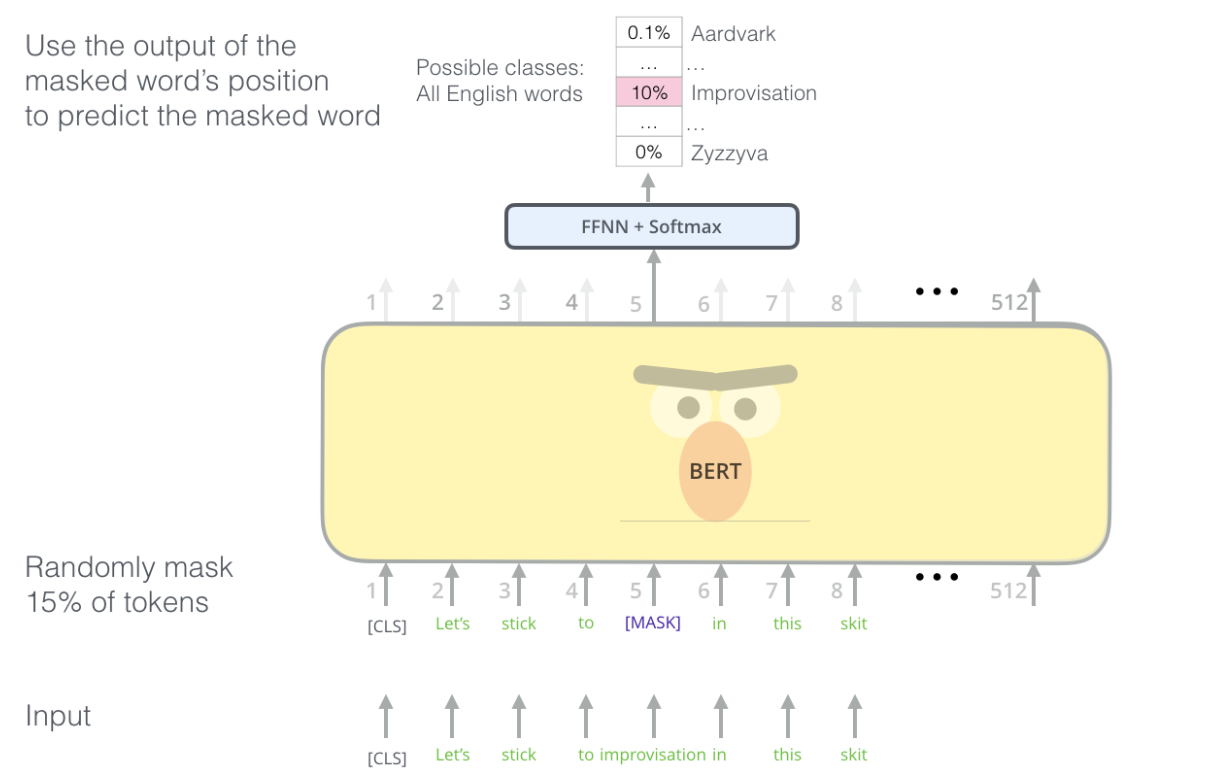
\includegraphics[width = 10cm]{figure/bert-mlm.png}\\ 
		\citebutton{Source: Jay Alammar}{https://jalammar.github.io/illustrated-bert/}
	\end{figure}

\vfill

\end{frame}

% ------------------------------------------------------------------------------

\begin{frame}{Next Sentence Prediction (NSP)}

\begin{itemize}
\item \textbf{Training objective:} $$\text{Given two sentences, predict whether $s_2$ follows $s_1$}$$
\item \textbf{Generation of samples:} $$\text{Randomly sample* negative examples (cf. word2vec)}$$
  \scriptsize *50\% of the time the second sentence is the actual next sentence, 50\% of the time it is a randomly sampled sentence
\item \normalsize \textbf{Full Input:}\\\mbox{}\\
			\footnotesize
\begin{center}
\begin{tabular}{|cccccccc|}
\hline
\cellcolor{blue!15}\texttt{[CLS]} & The & \cellcolor{blue!65}\texttt{[MASK]} & is & quick & . & \cellcolor{blue!15}\texttt{[SEP]} &\\\hline\hline It & jumps & over & the & \cellcolor{blue!65}\texttt{[MASK]} & dog & . & \cellcolor{blue!15}\texttt{[SEP]} \\
\hline
\end{tabular}\\\mbox{}
\end{center}
\item \normalsize \texttt{[CLS]} token as sequence representation for classification
\item \texttt{[SEP]} token for separation of the two input sequences
\end{itemize}

\end{frame}

% ------------------------------------------------------------------------------

\begin{frame}{NSP (2)}

\vfill

	\begin{figure}
		\centering
		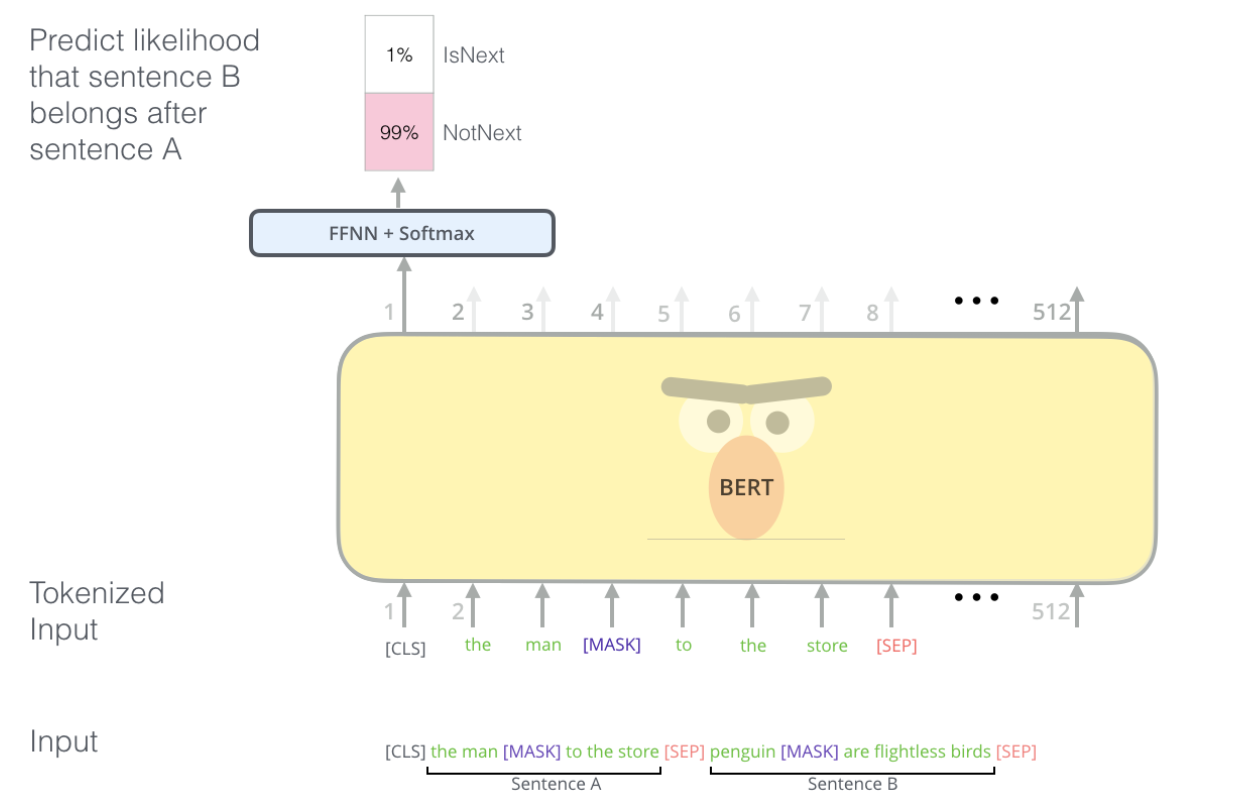
\includegraphics[width = 10cm]{figure/bert-nsp.png}\\ 
		\citebutton{Source: Jay Alammar}{https://jalammar.github.io/illustrated-bert/}
	\end{figure}

\vfill

\end{frame}

% ------------------------------------------------------------------------------

\begin{frame}{Pre-Training BERT}

\vfill

\textbf{Setup:}

\begin{itemize}
	\item 13 GB of text (BooksCorpus $+$ Eng. Wikipedia)\\
				$\rightarrow$ Back then: \textbf{huge}; Now: rather \textbf{small}
	\item Train for approximately* 40 epochs
	\item 4 (16) \href{https://cloud.google.com/tpu/}{Cloud TPUs} for 4 days for the BASE (LARGE) variant
	\item Loss function: $$Loss_{BERT} = Loss_{MLM} + Loss_{NSP}$$
\end{itemize}

\vfill

{\scriptsize *1.000.000 steps on batches of 256 sequences with a sequence length of 512 tokens}
\end{frame}

% ------------------------------------------------------------------------------

\begin{frame}{Pre-Training BERT}

\vfill

\textbf{Sequence lengths:}

\begin{itemize}
	\item For their experiments:
		\begin{itemize}
			\item Pre-train w/ sequence length 128 for 90\% of the steps
			\item Pre-train w/ sequence length 512 for 10\% of the steps \\
		\end{itemize}
	\item \textit{Reason:} Positional embeddings
		\begin{itemize}
			\item Learned, not sinusoidal (as opposed to the original Transformer)
			\item Training on long sequences necessary to learn them well
			\item \textbf{But:} Training expensive, hence this ``compromise``
		\end{itemize}
\end{itemize}

\vfill

\end{frame}

% ------------------------------------------------------------------------------

\begin{frame}{Fine-Tuning BERT}
	\begin{figure}
	\centering
		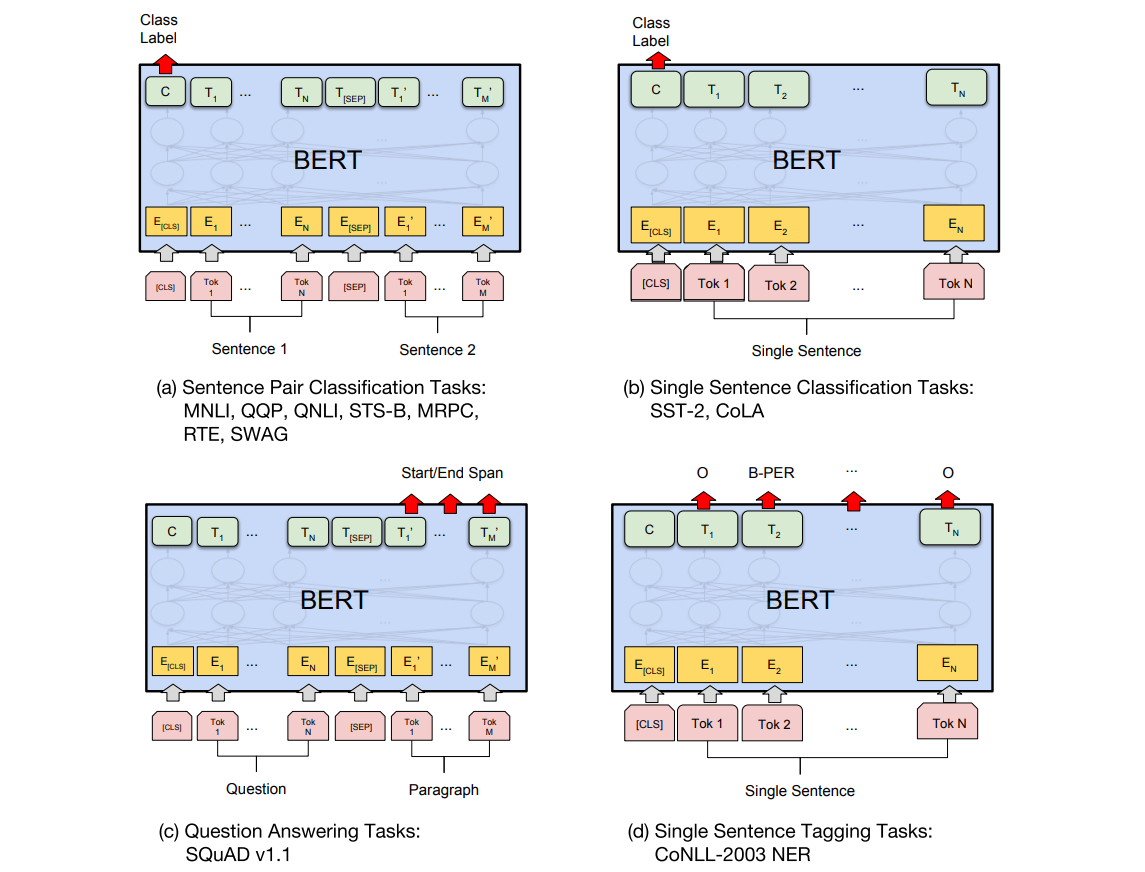
\includegraphics[width = 10cm]{figure/bert-finetune.png}\\ 
	\citebutton{Source: Devlin et al., 2019}{https://aclanthology.org/N19-1423.pdf}
	\end{figure}
\end{frame}


% ------------------------------------------------------------------------------

\begin{frame}{Fine-Tuning BERT}

\vspace{1.5cm}

	\begin{figure}
	\centering
		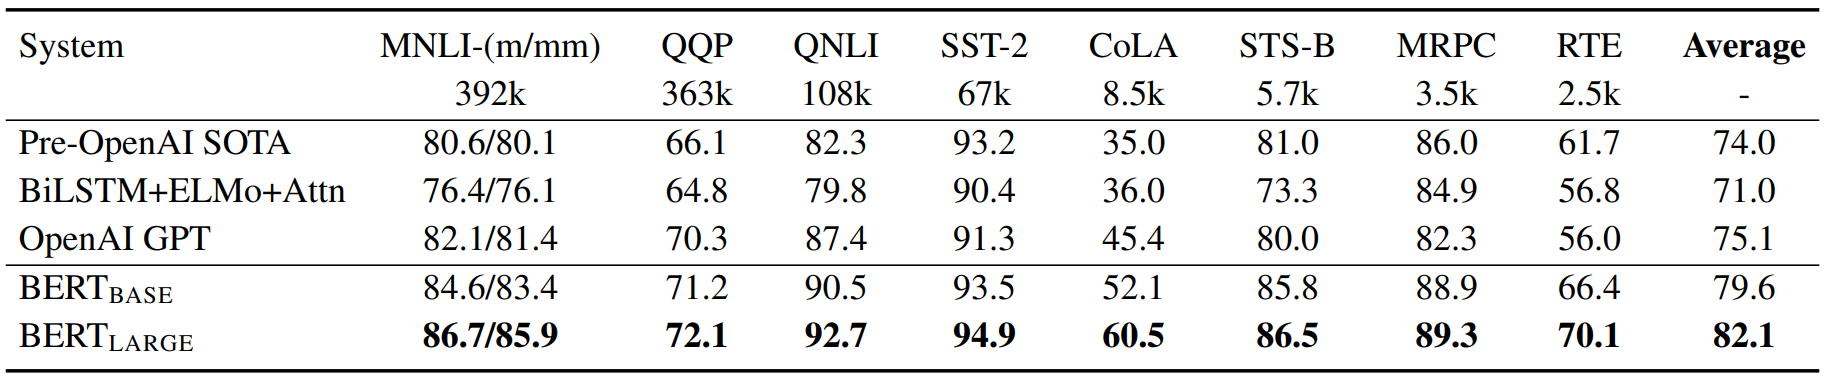
\includegraphics[width = 11cm]{figure/bert-sota.png}\\ 
	\citebutton{Source: Devlin et al., 2019}{https://aclanthology.org/N19-1423.pdf}
	\end{figure}
\begin{itemize}
	\item Performance of BERT on the GLUE Benchmark \citebutton{Wang et al., 2018}{https://gluebenchmark.com/}
	\item Beats all of the previous state-of-the-art models
	\item In the meantime: Other models (way) better than BERT
\end{itemize}

\end{frame}

% ------------------------------------------------------------------------------

\begin{frame}{Fine-tuning details}

\vfill

\begin{itemize}
	\item Relatively cheap compared to pre-training:
		\begin{itemize}
			\item $<$ 1 hour on a single Cloud TPU
			\item "a few hours" on a GPU
		\end{itemize}
	\item Recommendations for hyperparameters:
		\begin{itemize}
			\item \textbf{Batch Size:} 16, 32
			\item \textbf{Adam learning rate:} 5e-5, 3e-5, 2e-5
			\item \textbf{\#epochs:} 2, 3, 4
			\item \textbf{Dropout probability:} 0.1
		\end{itemize}
	\item Data sets w/ > 100k labeled examples rather insensitive to hyperparameters
\end{itemize}
	
\vfill

\end{frame}

% ------------------------------------------------------------------------------

\begin{frame}{Feature Extraction from BERT}

\vfill

	\begin{figure}
		\centering
		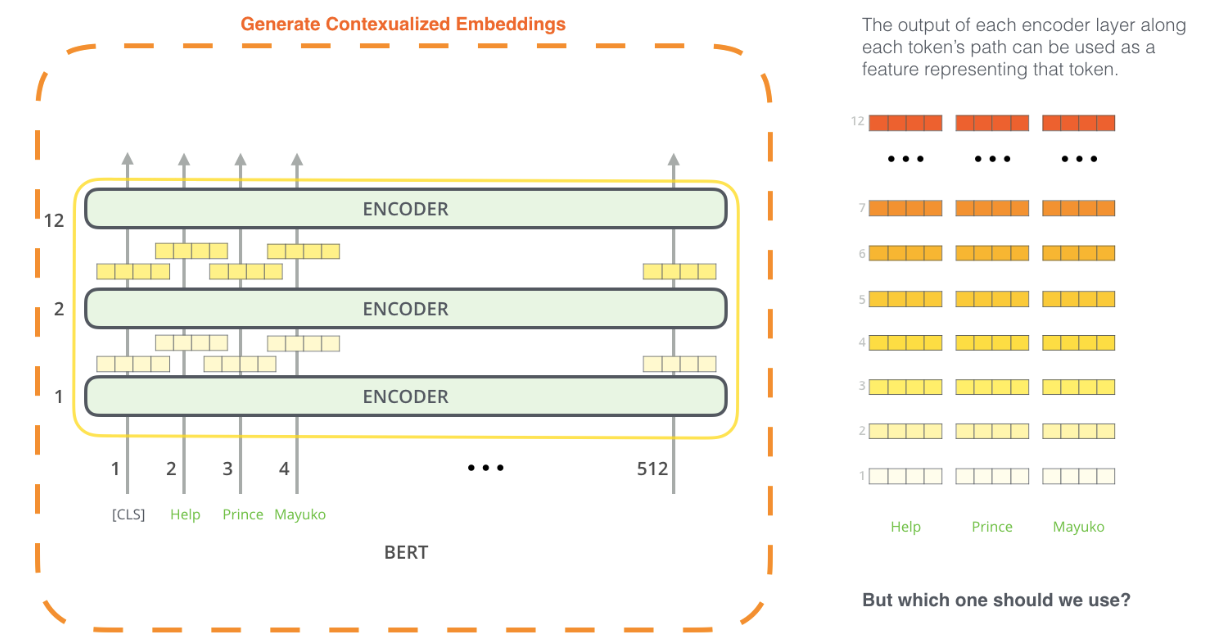
\includegraphics[width = 11cm]{figure/bert-featextr.png}\\ 
		\citebutton{Source: Jay Alammar}{https://jalammar.github.io/illustrated-bert/}
	\end{figure}

\vfill

\end{frame}

% ------------------------------------------------------------------------------

\begin{frame}{Feature Extraction from BERT}

	\begin{figure}
	\centering
		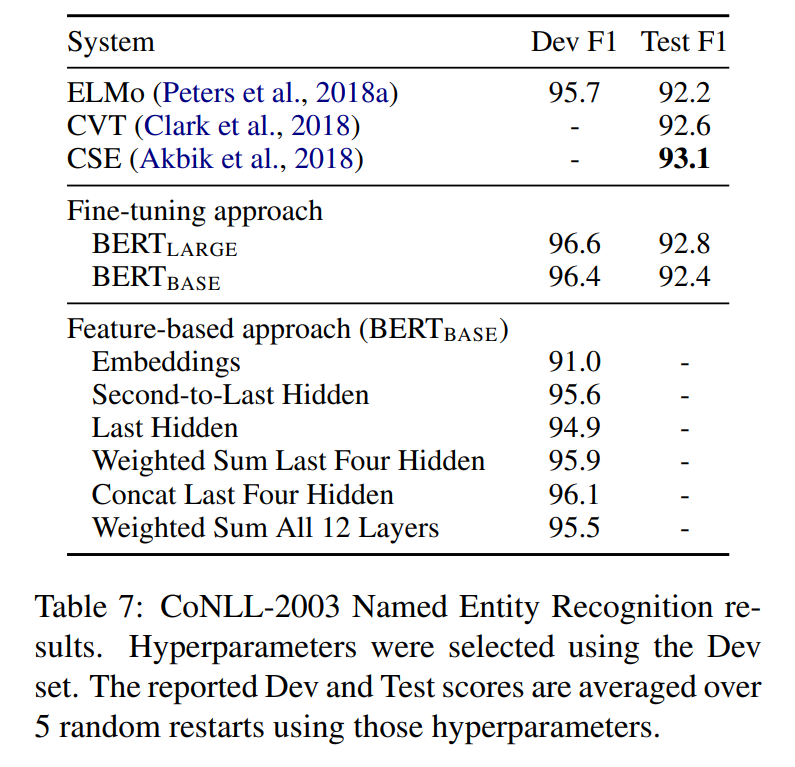
\includegraphics[width = 7.5cm]{figure/bert-featextr-results.png}\\ 
	\citebutton{Source: Devlin et al., 2019}{https://aclanthology.org/N19-1423.pdf}
	\end{figure}

\end{frame}

% ------------------------------------------------------------------------------

\endlecture
\end{document}
